\documentclass[12pt, a4paper]{article}
\usepackage{amsmath, amsfonts}
\usepackage[utf8]{inputenc}
\usepackage[russian]{babel}
\usepackage{graphicx}
\usepackage{tikz}
\usepackage{xcolor}
\usepackage{wrapfig}
\usepackage{float}
\usepackage{geometry}
\usepackage[indentfirst,compact,topmarks,calcwidth,pagestyles]{titlesec}
\usepackage{verbatim}
\usepackage{titletoc}
\usepackage{cmap}
\textheight=24cm
\textwidth=16cm
\oddsidemargin=5mm
\evensidemargin=-5mm
\marginparwidth=36pt
\topmargin=-1cm
\footnotesep=3ex
\raggedbottom
\tolerance 3000
\clubpenalty=10000
\widowpenalty=10000
\usepackage[T2A]{fontenc}
\usepackage{hyperref}

\newcommand\todo[1]{\marginpar{\textcolor{red}{#1}}}
\DeclareMathOperator*{\argmax}{argmax}
\DeclareMathOperator{\weight}{weight}
\DeclareMathOperator{\score}{score}
\DeclareMathOperator{\simu}{sim}

\begin{document}
  \section{Введение}
  	В современном мире информация быстро устаревает, поэтому способы вовремя находить нужные данные --- постоянный объект для исследований. Одним из направлений в этой области является извлечение данных из микроблоггинговых платформ.
  	
  	Платформы микроблогов стали очень популярным способом размещения данных в Сети. В них можно найти сообщения пользователей практически на любую тему, начиная стихийными бедствиями и заканчивая рейтингами музыкальных исполнителей. Правильная обработка доступной информации --- нетривиальная задача, которая имеет множество областей применения. Последние несколько лет эта тема активно исследуется во многих университетах мира.
  	
	Отслеживание сообщений о стихийных бедствиях в реальном времени поможет вовремя организовать спасательные операции и сохранить жизни людей\cite{nuggets}. Руководствуясь сообщениями пользователей микроблогов можно судить о популярности товаров и вовремя принимать экономически целесообразные решения. Можно делать предположения о рейтингах политических деятелей и эффективности рекламы на основании информации в микроблогах. Помимо перечисленных способов применения доступной информации в микроблоггинговых платформах можно привести множество других.
	
	В данной работе в дальнейшем будет рассматриваться сервис микроблогов Твиттер\footnote{http://www.twitter.com}. В нем помимо текстовой информации можно публиковать фото, видео и геотеги, что так же может быть использовано при анализе, но в этой работе не рассматривается. В доступном наборе данных можно проводить анализ разных сущностей, эта работа посвящена выявлению событий среди потоков информации. Поскольку трактовка событий в сообщениях микроблогов может быть субъективной, выделим несколько свойств, которыми характеризуется событие.
	
	Событие в первую очередь должно быть чем-то аномальным на фоне остальных данных. Оно определяется резким изменением частотных характеристик некоторых слов в сообщениях. События в микроблогах носят взрывной характер, в течении нескольких часов частоты релевантных слов возрастают в десятки раз и так же быстро опускаются до нормального уровня. Примером события могут быть: стихийное бедствие, выход спорного законопроекта на резонансную тему, получение фильмом награды на кинофестивале.
	
	Исторически подходы к описанной задаче менялись, в следующем разделе будет рассмотрена формальная постановка задачи и эволюция способов ее решения.
	
  \section{Описание задачи}
	Цель данной работы состоит из нескольких частей:
\begin{itemize}
\item исследовать существующие подходы по извлечению событий из сети Твиттер,
\item исследовать возможность применения иерархического процесса Дирихле для решения описанной задачи,
\item разработать метод для извлечения событий на основе иерархоческого процесса Дирихле,
\item продемонстрировать работу алгоритма на реальных данных.
\end{itemize}	  
  
  Объект изучения этой работы --- алгоритм, который по входным данным строит множество событий. В качестве данных для задач подобного рода служит мультимножество документов (сообщений):
\begin{equation}
  \Omega = \left\{D_i \,\vert\, i \in \overline{1,n} \right\}.
  \end{equation}  
  Будем считать, что каждый документ имеет временную метку $t$. Документ $D_i$ определяется как упорядоченный набор слов:
\begin{equation}
  D_i = \left\{w_j \,\vert\, j \in \overline{ 1, l_i } \right\},
  \end{equation}  
   при этом слова в документах принадлежат некоторому словарю $V$. 
  
  Событие --- некоторая сущность, которая характеризуется временем возникновения и ключевыми словами. Оно вызывает резкий подъем частотных характеристик некоторых слов. Событием может быть футбольный матч и музыкальный концерт. В социальной сети Твиттер есть популярные темы, которые всегда содержат много сообщений. Например это сообщения с ключевыми словами iphone и ipad. Но такие сообщения нельзя считать событиями. Также событиями нельзя считать еженедельные пятничные сообщения о конце рабочей недели\cite{waim13}.
  
  Особенности социальной сети Твиттер состоят в следующем:
  \begin{itemize}
  \item короткие сообщения (до 140 символов),
  \item наличие шума и ошибок,
  \item большая плотность сообщений.
  \item взрывной характер событий,
  \end{itemize}
  
  \section{Обзор существующих подходов}
  \subsection{NED}
  \label{ned-subsection}
	Исторически первым подходом к извлечению событий принято считать NED (New Event Detection)\cite{ned}. NED предназначен для того, чтобы находить первый документ на тему, которая не встречалась раньше. Следующие документы на эту тему уже не будут новыми и не будут помечены алгоритмом. Для того, чтобы отвечать на вопрос, является ли документ новым, необходимо указать способ как определять степень сходства двух документов.
	
\begin{figure}[H]
  \centering
  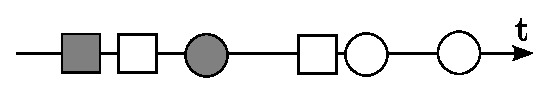
\includegraphics[width=0.58\textwidth]{ned.eps}
  \\
  \caption{Документы, соответствующие двум разным темам. Новые документы помечены серым цветом.}
  \end{figure}  

	Для этого в алгоритме NED используется техника Incremental TF--IDF (Term Frequency -- Inverse Document Frequency). TF--IDF --- базовый метод выяснять насколько отдельно взятые слова характеризуют весь документ, другими словами, насколько большой вес имеет слово $w$ в документе $d$. Пусть $f(d,w)$ --- количество слов $w$ в документе $d$. Определим значение $df_t(w)$ как количество документов, поступивших не позднее времени $t$, в которых встречается слово $w$. Используя введенные величины, можно записать значение веса определенного слова $w$ в документе $d$. В момент времени $t$ имеем:
	\begin{equation}
	\weight_t(d,w) = \frac{1}{Z_t(d)}f(d,w) \cdot \log \frac{N_t}{df_t(w)},
	\end{equation}
	где $N_t$ --- общее количество документов, поступивших не позднее времени $t$, $Z_t(d)$ --- нормализационное значение:
	\begin{equation}
	Z_t(d) = \sqrt{\sum_w \left[ f(d,w) \cdot \log \frac{N_t}{df_t(w)} \right]^2}
	\end{equation}.
	
	Теперь можно записать значение похожести двух документов, $q$ и $d$:
	\begin{equation}
	\simu_t(d,q) = \sum_w \weight(w, d) \cdot \weight(w, q).
	\end{equation}
	Указанные формулы записаны в косинусной метрике, также могут быть использованы метрики Хеллингера, Кульбака--Лейблера и другие.
	
	Для того, чтобы понять, является ли добавленный в момент времени $t$ документ $q$ новым, необходимо вычислить степень его похожести со всеми предыдущими документами. Пусть $d^*$ --- документ, максимально похожий на $q$:
	\begin{equation}
	d^* = \argmax_d \simu_t (d,q).
	\end{equation}
	Тогда значение
	\begin{equation}
	\score_t(q) = 1 - \simu_t (d^*, q)
	\end{equation}
	может быть использовано для того, чтобы определить, является ли документ $q$ новым. Новыми будем считать все документы $q$, у которых значение $\score_t(q)$ больше, чем пороговое значение $\theta_s$. В обратном случае считается что существует документ $d^*$, достаточно похожий на $q$ и поэтому $q$ не представляет собой сообщение на новую тему. Для того, чтобы определить подходящее значение $\theta_s$, можно использовать размеченный корпус и посчитать значение $\simu_t (d,q)$ среди документов, соответствующих одному и разным событиям.
	
	\subsection{Выявление событий с помощью LDA}
  На следующем примере рассмотрим как тематические модели (Topic Models) могут быть использованы для задачи распознавания событий. Для этого опишем схему, по которой работает алгоритм, предложенный в \cite{mediaeval}. Задача состоит в том, чтобы по данным к фотографиям Flickr\footnote{http://flickr.com} распознать все события на определенную тему, проходившие в конкретных городах. Фотографии содержат описания, которые можно считать документами. Основная задача может быть разбита на пять частей: 
  \begin{enumerate}
  \item предобработка данных,
  \item извлечение города,
  \item распознавание темы,
  \item распознавание события,
  \item оптимизация описания события.
  \end{enumerate}
  
  В качестве предобработки, авторы предлагают выполнить следующее: удалить стоп-слова и html теги, провести стемминг слов\footnote{стемминг (stemming) --- удаление окончаний у слов}, перевести не английские слова на английский язык используя сервис Google Translate.
  
	Так как задача упоминает отдельные города, необходимо научиться распознавать город по документу. Географические координаты были доступны авторам в 20\% фотографий, из этих координат были выявлены города используя сервис Google Tables. Используя технику TF--IDF, в описаниях фотографий с известными городами были извлечены ключевые слова. По этим ключевым словам, появилась возможность назначить фотографиям без геотегов "ближайший" город с точки зрения похожести описаний. Для того чтобы определять похожесть документов, можно воспользоваться подходом, описанным в~(\ref{ned-subsection}). В случаях, когда "ближайший" город выявить не удалось, авторами использовались следующие предположения: считалось что один и тот же автор не мог побывать в один день более чем в двух разных городах, и что путешествие из одного города в другой занимает как минимум два часа. Эти эвристики позволили улучшить классификатор, таким образом более 97\% фотографий были привязаны к городу.
	
	Далее необходимо для каждого города кластеризовать документы по темам и рассмотреть только те из них, которые даны в описании задачи. Для распознования тем была использована тематическая модель LDA (Latent Dirichlet Allocation)\cite{lda-model}, для определения параметров которой применялось сэмплирование по Гиббсу\cite{lda-gibbs}. LDA работает из предположения, что каждый документ $d_i$ характеризуется случайным распределением над темами, в то время как каждая тема является мультиномиальным распределением над словами.
	
	Оставшаяся часть --- извлечение событий и их оптимизация. Для того чтобы алгоритм выявил событие, отвечающее теме $k$ в день $D$, необходимо чтобы количество документов $d_i$ по этой теме в день $D$ превосходило некоторое пороговое значение $\theta$. Оптимизация событий подразумевает под собой объединение событий на одну тему в последовательные дни и разделение событий в разных городах.
	
	Авторы статьи тестировали алгоритм на трех разных вариантах условия задачи, в таблице ниже приведены результаты по каждому из них:
	
\begin{center}
    \begin{tabular}{| l | l | l | l | }
    \hline
    Данные & Точность & Полнота & F1-мера \\ \hline
    \#1 & 80.98 & 19.25 & 31.10 \\ \hline
    \#2 & 91.21 & 77.85 & 84.00  \\ \hline
    \#3 & 90.76 & 81.91 & 84.00 \\
    \hline
    \end{tabular}
\end{center}
  
  \section{Полученные результаты}
  В качестве данных были использованы сообщения пользователей Twitter с 4 июня 2013 года по 31 июня 2013 года, содержащие в себе хэштег \#texas. Всего корпус включает порядка 240 тысяч сообщений и 1.5 миллиона слов. 
  \section{Заключение}

\begin{thebibliography}{9}
	\bibitem{nuggets}
	Imran, Elbassuoni, Castillo, Diaz and Meier.
	Extracting Information Nuggets from Disaster-Related Messages in Social Media.
	2013.
	\bibitem{waim13}
	Xun Wang, Feida Zhu, Jing Jiang, Sujian Li.
	Real Time Event Detection in Twitter.
	2011.
	\bibitem{ned}
	Thorsten Brants, Francine Chen, Ayman Farahat.
	A System for New Event Detection.
	2003.
	\bibitem{mediaeval}
	Konstantinos N. Vavliakis, Fani A. Tzima, and Pericles A. Mitkas.	
	Event Detection via LDA for the MediaEval2012 SED Task.
	2012.
	\bibitem{lda-model}
	David M. Blei, Andrew Y. Ng, Michael I. Jordan.
	Latent Dirichlet Allocation.
	2003.
	\bibitem{lda-gibbs}
	Tom Griffiths.
	Gibbs sampling in the generative model of Latent Dirichlet Allocation.
\end{thebibliography}
  
\end{document}
